\documentclass{tufte-handout}
\usepackage{microtype}
\usepackage{tikz}
\usepackage{booktabs}
\input{vc.tex}  % For version control
\title{Disjoint Sets IV -- Move}
\author{}
\date{\GITAuthorDate, rev. \GITAbrHash}

\begin{document}
\maketitle
%\section{}
%\subsection

\begin{abstract}
  Maintain a family of disjoint sets under repeated operations that perform  unions of sets or move single elements from one set to another, using a tailor-made variant of a Union--Find data structure.

  To solve this exercise, you need construct a new data structure, instead of just taking a well-known solution off the shelf, as we did for Disjoint Sets II, or slighly extending a well-known solution, as we did for Disjoint Sets III.
  In other words, this is a data structure \emph{design} question, not an \emph{application} question.
\end{abstract}

\section{Description}
\begin{marginfigure}
  \begin{tabular}{ll}
    \texttt{4 9}   & $\{0\}, \{1\}, \{2\},\{3\}$\\
    \texttt{q 0 1} \\
    \texttt{u 0 1} & $\{0, 1\}, \{2\},\{3\}$ \\
    \texttt{q 0 1} &\\
    \texttt{u 1 2} & $\{0, 1, 2\},\{3\}$ \\
    \texttt{q 1 2} &\\
    \texttt{q 0 3} &\\
    \texttt{m 2 3}   & $\{0, 1\}, \{2,3\}$ \\
    \texttt{q 0 1} &\\
    \texttt{q 1 2} &
  \end{tabular}
  \caption{Sample input and interpretation.}
\end{marginfigure}

\begin{marginfigure}
  \begin{verbatim}
no
yes
yes
no
yes
no
  \end{verbatim}
  \caption{Sample output}
\end{marginfigure}

Maintain a family of disjoint sets, initially the singletons
\[ \{0\},\{1\}, \ldots,\{n-1\} \]
under the following operations:
\begin{description}
  \item[union]
The \emph{union} operation takes two arguments $s$ and $t$ and creates the union of the two sets containing $s$ and $t$.
More precisely, if $s\in S$ and $t\in T$ with $S\neq T$ then $S$ and $T$ are removed from the family and replaced by the set $S\cup T$. 
    (If $S=T$  then nothing happens.)
  \item[query]
    The \emph{query} operation takes two arguments $s$ and $t$ and determines if $s$ and $t$ belong to the same set.
    More precisely, if $s\in S$ and $t\in T$ then print \texttt{yes} if $S=T$ and print \texttt{no} if $S\neq T$.
  \item[move]
    The \emph{move} operation takes two arguments $s$ and $t$ and moves the element $s$ to the set containing $t$, removing $s$ from whatever set it may have belonged to before.
    More precisely, if $s\in S$ and $t\in T$ with $S\neq T$ then $S$ and $T$ are removed from the family and $S-\{s\}$ (if it is nonempty)  and $T\cup\{s\}$ are added to the family.
    (If $S= T$ then nothing happens.)
\end{description}
Note that these operations maintain invariantly that the sets in the family are disjoint.
The meaning of the union and query operations is exactly as in \emph{Disjoint Sets I} and \emph{Disjoint Sets II}.

\subsection{Input}

The input starts with two nonnegative integers $n$, $m$, on the first line.
We have $0\leq n\leq 10^6$ and $0\leq m\leq 2\cdot 10^6$.
The integer $n$ is the initial number of singletons.
The following $m$ lines are of the form ``\texttt{u} $s$ $t$'' (for \emph{union}) or ``\texttt{q} $s$ $t$'' (for \emph{query}) or ``\texttt{m} $s$ $t$'' (for \emph{move}); you can assume $0\leq s< n$ and $0\leq t< n$.

\subsection{Output}

For each query, a single line with \texttt{yes} or \texttt{no} as described above.

\section{Deliverable}

\begin{description}
  \item[Source code of solution.]
    Solve the problem in Python or Java.
    Hand this in as \texttt{Ds4.java} or \texttt{ds4.py}.

    There is a set of instances on CodeJudge for you to test.
  \item[Report.]
    Hand in a very brief report describing your data structure as a PDF. 
    The solution should pass all tests on the Code Judge, and your report should say this and mention the resulting running times.
    \textbf{Please add the number of the successful submission on Code Judge to your report.}
    Please include all the names and itu-email addresses of the group members as authors in the PDF of the report.
\end{description}

This is a difficult exercise because the standard Union--Find data structures you can find in libraries or text books will not solve it.
(A moment's thought should convince you that the move operation can destroy the trees built in in the standard Union--Find data structure, typically when $s$ is not a leaf in the data structure.)
On the other hand, the instances are so large that an efficient solution is necessary.

A good idea is needed, and your report should explain it briefly and clearly.
A figure is probably useful.
(Draw it by hand and scan it, unless you are really familiar with some good drawing tools.)

Your solution must use at most logarithmic time (in $n$) per update, and total space linear in $n$.

\newpage
\section{Disjoint Sets IV Report}

by Alice Cooper, Bob Marley, and Charlie Brown\sidenote{Complete the report by filling
  in your real name and changing other parts wherever necessary.
  Remove the sidenotes in your final hand-in.}

  
  We solved this exercise in Python 3 / Java.

  Program \texttt{ds4} passes all tests on the CodeJudge, with a maximum of running time of 4 seconds.

  \medskip

  Our data structure is a modification of Weighted Max Flow\sidenote{The description, including the illustration, is utter nonsense and just here to indicate how many sentences you should roughly use. Replace the nonsense.} 
  except that we also maintain a homeotoxic metasnail for every inverse tachyon flux capacitator.
  (As in [SW, sec. 1.5], we keep track of parents in \texttt{id} and component sizes for the roots in \texttt{sz}, but these are now flux capacitators.)

  Queries and unions are almost the same as in the standard solution, except for the extra step of subverting the flux capacitator.
  For $\emph{move}(s,t)$, a new copy of the node is inserted in the particle reference queue, and the nunstuck is popped.

  \medskip
  
  For instance, just before the move operation in the sample input, the data structure looks like this:

 \begin{figure}[h]
   \begin{minipage}{3cm}
     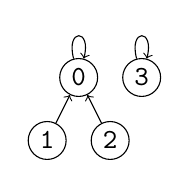
\begin{tikzpicture}[scale = .8]
    \node (0) at (  0,  0) [draw, inner sep = 2pt, circle] {\texttt{0}};
    \node (1) at (-.5, -1) [draw, inner sep = 2pt, circle] {\texttt{1}};
    \node (2) at (+.5, -1) [draw, inner sep = 2pt, circle] {\texttt{2}};
    \node (3) at (  1,  0) [draw, inner sep = 2pt, circle] {\texttt{3}};
    \draw [->] (1)--(0);
    \draw [->] (2)--(0);
    \draw [->] (0) to [loop above] (0);
    \draw [->] (3) to [loop above] (3);
  \end{tikzpicture}
   \end{minipage}
  \qquad
   \begin{minipage}{4cm}
   \begin{tabular}{lcccc}
     element & \texttt{0} & \texttt{1} & \texttt{2} & \texttt{3} \\  \midrule
     \texttt{id}         & \texttt{0} & \texttt{0} & \texttt{3} \\
     \texttt{sz}         & \texttt{3} &  -- & -- & \texttt{1} \\
     \texttt{flux}    & $\pi$ \\ 
   \end{tabular}
   \end{minipage}
 \end{figure}

  After the move, element $2$ is again just a reference to the inverse flux capacitator, and its old tachyon node remains untouched.

 \begin{figure}[h]
   \begin{minipage}{3cm}
     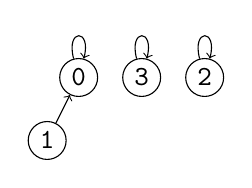
\begin{tikzpicture}[scale = .8]
    \node (0) at (  0,  0) [draw, inner sep = 2pt, circle] {\texttt{0}};
    \node (1) at (-.5, -1) [draw, inner sep = 2pt, circle] {\texttt{1}};
    \node (2) at (  2,  0) [draw, inner sep = 2pt, circle] {\texttt{2}};
    \node (3) at (  1,  0) [draw, inner sep = 2pt, circle] {\texttt{3}};
    \draw [->] (1)--(0);
    \draw [->] (2) to [loop above] (2);
    \draw [->] (0) to [loop above] (0);
    \draw [->] (3) to [loop above] (3);
  \end{tikzpicture}
   \end{minipage}
  \qquad
   \begin{minipage}{4cm}
   \begin{tabular}{lcccc}
     element & \texttt{0} & \texttt{1} & \texttt{2} & \texttt{3} \\  \midrule
     \texttt{id}         & \texttt{0} & \texttt{2} & \texttt{3} \\
     \texttt{sz}         & \texttt{3} &  -- & -- & \texttt{1} \\
     \texttt{flux}    & $2\pi$ \\ 
   \end{tabular}
   \end{minipage}
 \end{figure}


 \medskip
  We claim without proof
  \footnote{If you want, you can give a proof. This is not mandatory.}
  that the running time is logarithmic in $n$ in the worst case per update and the data structure requires linear space in  $n$ space.
\end{document}
